\documentclass[border=4pt]{standalone}
\usepackage{tikz}
\usetikzlibrary{automata, positioning, arrows}
\tikzset{->,  % makes the edges directed
	>=stealth, % makes the arrow heads bold
	node distance=3cm, % specifies the minimum distance between two nodes. Change if necessary.
	every state/.style={thick, fill=blue!10}, % sets the properties for each ’state’ node
%	minimum size=2.5cm,
	initial text=$ $, % sets the text that appears on the start arrow
}
\begin{document}
	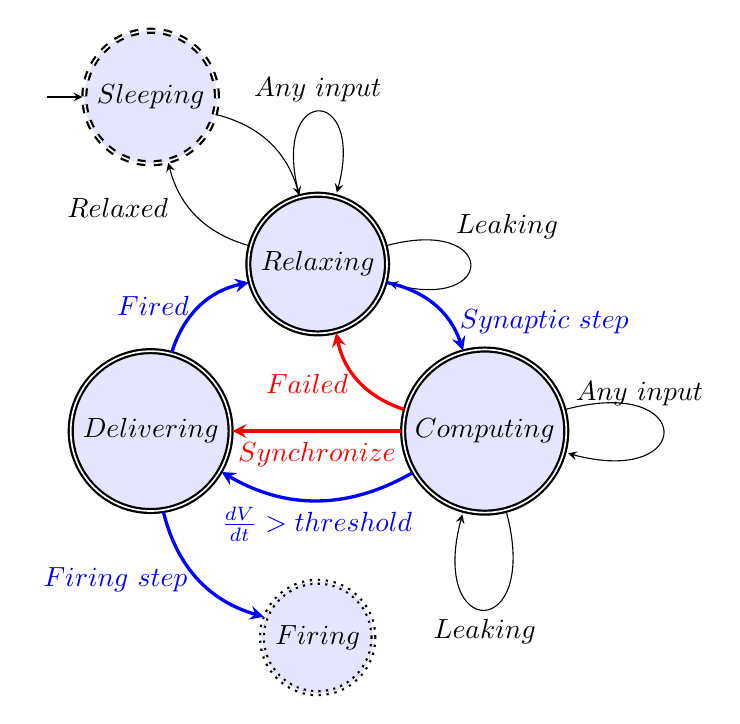
\begin{tikzpicture}
	% Initially, the neurer is ready, but sleeping
	\node[state, accepting, initial, dashed, thick] (Sleeping) {$Sleeping$};
	% The major state is 
	\node[state, accepting, below right of=Sleeping] (Relaxing) {$Relaxing$};
	\draw (Sleeping) edge[bend left,xshift=.5cm,yshift=-.5cm] node{} (Relaxing) ;
	\draw   (Relaxing) edge[loop above] node[above]{$Any~input$} (Relaxing);	
	\draw   (Relaxing) edge[loop right] node[above right, yshift=.2cm, xshift=-0.3cm]{$Leaking$} (Relaxing);	
	\node[state,  accepting, below right of=Relaxing] (Computing) {$Computing$};
	\draw   (Computing) edge[loop below] node[]{$Leaking$} (Computing);	
	\draw   (Computing) edge[loop right] node[above, yshift=.2cm, xshift=-0.3cm]{$Any~input$} (Computing);	
	%% Make a synaptic step
	\draw (Relaxing) edge[bend left, above left, color=blue, very thick] node[ xshift=2.6cm,yshift=-.5cm]{$Synaptic\ step$} (Computing) ;	
	\draw (Computing) edge[bend left, above left, color=red, very thick] node[yshift=-0.3cm]{$Failed$} (Relaxing) ;
	
	%% Will fire, somehow
	\node[state, accepting, below left of=Relaxing] (Delivering) {$Delivering$};
	%% in steps:
	\node[state, accepting, below right of=Delivering, yshift=-.5cm, dotted] (Firing) {$Firing$};
	\draw (Delivering) edge[bend right, above left, , color=blue, very thick] node[yshift=-0.3cm]{$Firing\ step$} (Firing) ;	
	
	

	\draw (Computing) edge[ bend left, color=blue, very thick] node[ yshift=-.3cm
]{$\frac{dV}{dt}>{threshold}$} (Delivering) ;
	\draw (Computing) edge[ color=red, very thick] node[yshift=-0.3cm]{$Synchronize$} (Delivering) ;

	\draw (Delivering) edge[bend left, color=blue, very thick] node[xshift=-.6cm 
]{$Fired$} (Relaxing) ;
	
	\draw (Relaxing) edge[bend left] node[
yshift=.1cm, xshift=-1cm
]{$Relaxed$} (Sleeping) ;
%	\node[state, initial] (q1) {$q_1$};
%	\node[state, accepting, right of=q1] (q2) {$q_2$};
%	\node[state, right of=q2] (q3) {$q_3$};
%	\draw   (q1) edge[loop above] node{0} (q1)
%	(q1) edge[above] node{1}
%	(q2)(q2) edge[loop above] node{1} (q2)
%	(q2) edge[bend left, above] node{0} (q3)
%	(q3) edge[bend left, below] node{0, 1} (q2);
	\end{tikzpicture}
\end{document}